\section{Preliminary}
\subsection{Background: Attention, KV cache, and Hardware-Aware Optimization} 

The attention mechanism \citep{transformer} is a core component of LLMs. Given an input sequence \( \mathbf{X} \in \mathbb{R}^{b \times s \times d} \), where \( b \) is the batch size, \( s \) is the sequence length, and \( d \) is the hidden dimension, it is first projected into \( \mathbf{Q} , \mathbf{K}, \mathbf{V} \) by learnable weight matrices \( \mathbf{W}_q, \mathbf{W}_k, \mathbf{W}_v \in \mathbb{R}^{d \times d} \). For simplicity, we omit the number of the attention heads.
The attention output is computed using the Scaled Dot-Product Attention mechanism as follows:
\begin{equation}
\label{eq:attention}
\resizebox{\columnwidth}{!}{$
\text{Attention}(\mathbf{Q}, \mathbf{K}, \mathbf{V}) = \text{softmax}\left(Mask(\frac{\mathbf{QK}^T}{\sqrt{d_k}})\right)\mathbf{V}
$}
\end{equation}
where $d_k$ is the dimension of the key vectors.
However, this attention mechanism relies on all past \(\mathbf{K} \) and \(\mathbf{V} \) when calculating the output of the current step. Therefore, LLMs typically utilize KV cache to accelerate auto-regressive decoding. The generation process of LLMs with KV cache is divided into the prefill phase and the decoding phase \citep{pd}.

\begin{figure}[t]
  \centering
  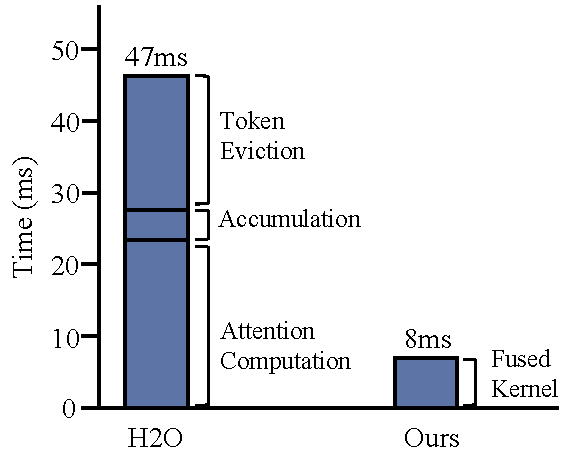
\includegraphics[width=0.4\textwidth]{figure/speed_kernel_cropped.pdf}
  \caption{Attention module latency of H2O and our kernel on Qwen3-8B with batch size 128 and sequence length 3200. Both methods evict one token after each attention computation.}
  \label{fig:speed_kernel}
\end{figure}


\textit{i)} During the prefill phase, given input \( \displaystyle \mX \), the Keys \( \displaystyle \mK_{<n} \) and Values \( \displaystyle \mV_{<n} \) are computed and cached.
\textit{ii)} During the decoding phase, only the Keys and Values of the new token \( x_n \) need to be calculated, which are then combined with the cached Keys and Values to execute attention computation.

From Equation \ref{eq:attention}, we can find that the classical attention computation is a memory-bound operation, as it requires multiple intermediate value accesses in HBM. Fortunately, Flash-Attention \cite{dao2022flashattention, dao2023flashattention2} uses IO-aware operations to minimize the number of read and write operations to HBM. By processing the computation in blocks (tiling) and leveraging on-chip SRAM to store intermediate results, Flash-Attention avoids materializing the full N×N attention score matrix in HBM. This dramatically reduces memory traffic, leading to significant speedups and a lower memory footprint. Inspired by this IO-aware approach, our custom kernel also employs a block-wise computation strategy to ensure maximum efficiency, as illustrated in Figure~\ref{fig:method}.


\subsection{Revisiting KV cache Compression in the Era of Long Reasoning Models}

While prior KV cache compression techniques have demonstrated considerable success in the traditional paradigm of long-input, short-output tasks, their core design assumptions are fundamentally challenged by the rise of long reasoning models. The shift to a long-output paradigm exposes several critical limitations in these established methods:

\noindent\textbf{Prefill-Only Compression.} Many methods are confined to the prefill stage, compressing only the initial prompt \citep{pyramidkv}. In long-output scenarios, where most of the tokens are generated during the decoding phase, this approach results in a drastically diminished compression ratio.



\noindent\textbf{High Computational and Memory Overhead.} Existing methods rely on token importance for eviction. The importance evaluation process is computationally expensive, adding significant latency to each compression step \citep{vatp,rkv}. Moreover, these methods often require storing auxiliary metadata, such as attention scores \citep{h2o} or past queries \citep{snapkv}, which consumes extra memory and partially cancels out the benefits of compression.

\noindent\textbf{Poor Compatibility with Modern Fused Kernels.} The performance of modern inference systems heavily relies on operator fusion like Flash-Attention \citep{dao2022flashattention,dao2023flashattention2} or Paged-Attention \citep{vllm}.
However, many compression algorithms are not compatible with these kernels.
Their logic can interrupt the fusion process, forcing data to be moved between SRAM and HBM, or they may require recalculating intermediate results that were already available during the attention step, which can make the overall inference process even slower.

These challenges require a complete redesign of KV cache compression based on the principles of dynamic applicability, lower overhead, and system-level implementation.